%% Octopus CPC paper
%% Template: Elsevier CAS single-column (cas-sc)
\documentclass[a4paper,fleqn]{cas-sc}

\usepackage[numbers,sort&compress]{natbib}
\usepackage{amsmath,amssymb}
\usepackage{mathtools}
\usepackage{booktabs}
\usepackage{graphicx}
\usepackage{array}
\usepackage{float}
\usepackage{placeins}

\AtBeginDocument{\hypersetup{
  pdftitle={GPU-accelerated framework for multi-slice strong-strong beam-beam simulation},
  pdfauthor={Derong Xu and Yi-Kai Kan},
  pdfsubject={Computer Physics Communications submission}}}

%% Convenience macros
\newcommand{\kbb}{k_{\mathrm{bb}}}
\newcommand{\code}[1]{\texttt{#1}}

\begin{document}
\let\WriteBookmarks\relax
\shorttitle{Octopus strong--strong beam--beam framework}
\shortauthors{D. Xu and Y.-K. Kan}

\title [mode = title]{GPU-accelerated framework for multi-slice strong--strong beam--beam simulation}
\author[1]{Derong Xu}[orcid=0000-0003-0396-4166]
\cormark[1]
\cortext[1]{Corresponding author}
\ead{dxu@bnl.gov}
\credit{Conceptualization, Methodology, Software, Validation, Formal analysis, Writing -- original draft, Writing -- review \& editing}

\author[1]{Yi-Kai Kan}

\affiliation[1]{organization={Brookhaven National Laboratory},
                city={Upton},
                state={New York},
                postcode={11973},
                country={United States}}

\begin{abstract}
Strong--strong beam--beam simulation must evolve two bunches self-consistently
while controlling field discretization, macroparticle noise, and computational
cost.  We present Octopus, a Julia/CUDA framework for multi-slice,
six-dimensional tracking whose common collision driver supports four
transverse field models, from a soft-Gaussian closure to full
particle-in-cell (PIC) solvers.  Two numerical developments address errors
exposed by adaptive PIC:
an assignment-consistent Gaussian/residual field split and node-indexed meshes
that remove the mesh-mismatch component of slice-boundary discontinuities.  An
ensemble analysis separates mean-field bias from finite-particle fluctuation
and shows that mesh refinement can reduce the former while increasing the
latter.  Validation progresses from structural identities and analytic fields
to Vlasov theory and the unmodified BeamBeam3D code.  At the tested settings,
PIC-family and BeamBeam3D round-beam coherent factors lie within 1.42\% of the
Vlasov reference, and the largest same-setting cross-code difference is
0.31\%.  A historical 15-slice, 8192-turn EIC application gives comparable
emittance evolution under nonidentical inputs.  Because complete source and
raw-output provenance was not retained, it is qualitative context rather than
source-pinned validation.  An EIC-scale case with
$3.58\times10^6$ macroparticles advances in about $0.31$~s per turn on one
NVIDIA RTX~4500 Ada GPU.  Together, the error analysis, validation, and timing
results support practical strong--strong studies within the tested domain.
\end{abstract}

\begin{keywords}
beam--beam interaction \sep strong--strong simulation \sep particle-in-cell \sep
GPU computing \sep accelerator physics \sep Julia
\end{keywords}

\maketitle

\makeatletter
\gdef\@pdfauthor{Derong Xu and Yi-Kai Kan}
\gdef\@pdftitle{GPU-accelerated framework for multi-slice strong-strong beam-beam simulation}
\gdef\@pdfsubject{Computer Physics Communications submission}
\makeatother

%% ===================================================================
\section{Introduction}
\label{sec:intro}

The beam--beam interaction is a fundamental luminosity limit in circular
colliders.  A weak--strong model freezes one beam as an analytic
distribution, whereas a strong--strong model evolves both bunches
self-consistently and is therefore required for coherent two-beam modes and
mutual emittance evolution.  The synchro-beam map of
\citet{HirataMoshammerRuggiero1993}, the strong--strong formulation of
\citet{Ohmi2000}, and the parallel PIC implementation in BeamBeam3D
\citep{Qiang2004BeamBeam3D,QiangGreen2002} established the numerical basis
for multi-slice circular-collider studies
\citep{OhmiTawadaEtAl2004,Stern2010,HerrPieloni2014,QiangBlaskiewicz2024}.
Their cost nevertheless remains substantial: every turn couples many slice
pairs, each requiring charge assignment, an open-boundary field solve, and
two particle gathers.

Octopus is a Julia \citep{BezansonJulia2017} framework with a CUDA backend
\citep{BesardCUDAjl2019} for this workload.  It combines six-dimensional
weak--strong tracking and multi-slice strong--strong collisions in one set
of conventions, with four field models behind one collision interface.
The production solver uses a fixed number of cells whose physical extent
adapts to each interacting pair.  Reduced beam--beam meshes
\citep{CaiReducedMesh2001}, Gaussian/residual ($\delta f$) decompositions
\citep{KogaTajima1995,CaiDeltaf2000}, and slice-endpoint potential
interpolation \citep{OhmiTawadaOide2003,KabelCai2004} are established.  The
numerical contributions here are narrower: an equal-weight full-$f$ field
splitting in which a live Gaussian reference is projected analytically
through the particle assignment operator, and the identification of a
mesh-consistency failure when adjacent slice pairs construct adaptive
transverse grids independently.  A node-indexed grid removes this
mesh-mismatch term while retaining live-source evolution.

Within the common GPU-oriented driver, the four solvers have distinct
production and diagnostic roles.  We evaluate them through a connected
sequence: field-error decomposition, analytic and BeamBeam3D collective tests,
a historical EIC emittance application, and production-scale timing.  The
source-pinned tests assess accuracy; the EIC application and timing establish
the physical and computational scope reached in practice.

Sections~\ref{sec:physics} and \ref{sec:methods} define the physics and
algorithms; Sections~\ref{sec:error} and \ref{sec:validation} analyze error and
validate collective observables.  Section~\ref{sec:cuda} reports performance,
followed by the conclusions.

%% ===================================================================
\section{Physics model and conventions}
\label{sec:physics}

\subsection{Coordinates and the coupling constant}
\label{sec:conventions}

Octopus tracks the canonical 6D coordinates $\mathbf q=(x,p_x,y,p_y,z,p_z)$,
with $z$ the longitudinal position relative to the reference particle
(positive toward the bunch head) and $p_z=(P-P_0)/P_0$ the relative momentum
deviation.  Beams are ultrarelativistic and counter-propagating; each
collision is decomposed into thin longitudinal slices, and each slice pair
interacts through a two-dimensional transverse potential.  All solvers share
one coupling constant per kicked beam,
\begin{equation}
  \kbb = q_1 q_2\, \frac{N r_0}{\gamma},
  \label{eq:kbb}
\end{equation}
where $q_{1,2}=\pm1$ are the charge signs, $N$ the source bunch population,
and $r_0$ and $\gamma$ the classical radius and Lorentz factor of the
\emph{kicked} species.  The transverse kick of a Gaussian slice of weight
$w$ is $\Delta\mathbf p_\perp = \kbb\, w\,\mathbf K_{\rm BE}$, where
$\mathbf K_{\rm BE}$ is the Bassetti--Erskine kick function normalized so
that $|\mathbf K_{\rm BE}|\to 2/r$ far from a round slice
\citep{BassettiErskine1980}.  With this
normalization the nominal beam--beam parameter is
$\xi_{x,y} = N r_0 \beta^*_{x,y}/[2\pi\gamma\,\sigma_{x,y}(\sigma_x+\sigma_y)]$
with the source beam's sizes, reducing to
$\xi = N r_0 \beta^*/(4\pi\gamma\sigma^2)$ for round beams; all $\xi$
values quoted in this paper are nominal (design $\sigma$), and the PIC kick is normalized per
deposited source macroparticle so that it reduces to
$\kbb w\,\mathbf K_{\rm BE}$ for a Gaussian slice.

\subsection{The synchro-beam map}
\label{sec:sbm}

A particle at longitudinal position $z$ colliding with a thin source slice at
$z_*$ meets it at the collision point $S=(z-z_*)/2$ along the particle's own
axis \citep{HirataMoshammerRuggiero1993}.  The collision map is the
composition $\mathcal M=\mathcal D^{-1}\mathcal B\,\mathcal D$ of a
\emph{virtual drift} $\mathcal D$ to the collision point, the thin transverse
kick $\mathcal B$, and the inverse drift, with maps composed
\emph{right to left} --- the rightmost factor $\mathcal D$ acts first.
Because the drift length depends on
the canonical coordinate $z$, symplecticity requires a compensating change of
$p_z$ --- the ``slingshot'' term.  For the default paraxial (Hirata) drift
with drift Hamiltonian $H=(p_x^2+p_y^2)/2$ the energy exchange is
\begin{equation}
  \Delta p_z^{\rm sling}
  =\frac{(p_x^+)^2+(p_y^+)^2-(p_x^-)^2-(p_y^-)^2}{4},
  \label{eq:sling}
\end{equation}
where superscripts $-$ and $+$ denote values before and after the transverse
kick, respectively.  Octopus also
provides chromatic and exact-Hamiltonian virtual drifts.

For a Gaussian strong source, the analytic longitudinal kick at the collision
point generalizes Hirata's formula to a moving source centroid and a fully
transported source covariance
$A=\begin{psmallmatrix} a & b\\ b & d\end{psmallmatrix}$, including the
transverse coupling $b=\sigma_{xy}$ \citep{LeunissenSchmidtRipken2000}.  Let
$u=-S$ denote the collision position measured along the \emph{source} axis,
and let
$\mathbf C(u)$ and $A(u)$ be the source centroid and covariance there.  All
charge and normalization factors are absorbed into the slice potential $U$,
with transverse kick $\mathbf F=-\nabla U$.  Since $z$ enters only through
$S$, symplecticity requires $\Delta p_z^{\rm CP}=-\partial U/\partial z$
evaluated at the collision point, and with $u_z=-1/2$ the Gaussian
heat-equation identity $\mathrm dU=\tfrac12 H_U\!:\!\mathrm dA$ (with
$H_U=\nabla\nabla U$ the transverse Hessian) gives the coordinate-invariant
form
\begin{equation}
  \Delta p_z^{\rm CP}
  = \tfrac12\,\mathbf F\cdot\mathbf C_u
  + \tfrac14\, H_U\!:\!A_u ,
  \label{eq:dpz}
\end{equation}
where $\mathbf C_u$ and $A_u$ are derivatives with respect to $u$.  The
Gaussian heat-equation identity is essential to this analytic form; PIC and
spectral routes obtain the corresponding longitudinal kick from numerical
potential differences.  In
principal axes Eq.~\eqref{eq:dpz} splits into centroid, principal-size, and
\emph{principal-axis rotation} contributions; the rotation term is
easily
omitted by models that rotate coordinates and forces correctly but treat the
tilt as frozen.  Eight analytic limits and the 6D symplecticity of the composed
map are tested in Section~\ref{sec:validation}.

\subsection{Source models and longitudinal slicing}
\label{sec:slicing}

The weak--strong source is a full 6D Gaussian specified by its $6\times6$
covariance.  Slices are obtained by \emph{conditional} (not projected)
slicing: writing $\mathbf w=(x,p_x,y,p_y)$ for the transverse block,
\begin{equation}
  \boldsymbol\mu_{w\mid z_i}=\boldsymbol\mu_w+\frac{\Sigma_{wz}}{\Sigma_{zz}}(z_i-\mu_z),
  \qquad
  \Sigma_{w\mid z}=\Sigma_{ww}-\frac{\Sigma_{wz}\Sigma_{zw}}{\Sigma_{zz}},
  \label{eq:conditional}
\end{equation}
so all delta slices of a joint Gaussian share one transverse covariance and
differ only in their 4D centroids.  This cleanly separates the two
dispersion-like couplings: linear crab dispersion moves slice centroids
without changing the conditional slice size, while momentum dispersion widens
and couples the within-slice covariance.

In the strong--strong task both beams are live macroparticle ensembles.  Each
beam is cut into $n$ longitudinal slices (equal-area, normal-quantile,
equal-width, or user-specified boundaries); slice pairs interact in
collision-time order, and the transverse kick, together with the longitudinal
kick obtained from analytic moments or potential differences, is applied to
both beams.  In the PIC path the field of a source slice is solved at
slice-boundary nodes and interpolated linearly (default) or quadratically in
$z$; the Gaussian-subtracted and spectral paths currently use linear
interpolation, whereas soft-Gaussian evaluates each particle directly.  In
all cases the transverse evaluation point is drift-transported to its
collision point.  Endpoint interpolation assumes that both sides of a slice
boundary represent the nominally shared node with the same discrete
transverse operator.  Independently adapted per-pair meshes violate that
assumption; Section~\ref{sec:nodemesh} describes the node-indexed alternative.

\subsection{Machine elements}

Between collisions, beams are tracked through linear 6D one-turn maps or
element sequences: multi-harmonic thin crab cavities, Hirata's crossing-angle
Lorentz boost pair \citep{Hirata1995}, chromaticity kicks, dispersion and
coupling maps, and a lumped radiation element applying damping and quantum
excitation in decoupled, dispersion-free coordinates.  Stochastic excitation
uses a counter-based Philox random number generator \citep{Salmon2011} keyed by
$(\text{seed},\text{turn},\text{stream},\text{particle},\text{component})$,
so the excitation is independent of CPU threading and CUDA launch geometry.
The crab-crossing collision geometry follows the EIC scheme
\citep{XuCrab2021,XuBB2024}.  Luminosity is accumulated per slice
pair as the discrete overlap integral
$L_{\rm pair}\propto (h_xh_y)^{-1}\sum_{ij} q^{(1)}_{ij}q^{(2)}_{ij}$,
where $q^{(1,2)}$ are the two slices' charges deposited on a shared
bounding grid of spacing $(h_x,h_y)$, normalized by macroparticle
weights and scaled by bunch populations and collision frequency ---
i.e.\ the standard mesh estimator of $\int\rho_1\rho_2\,dx\,dy$ per
colliding slice pair.  It uses the pre-collision live slice particles
transported to the collision midpoint.  Soft-Gaussian instead averages one
slice's analytic Gaussian density over the other slice's live midpoint
sample; it is not a closed-form Gaussian--Gaussian overlap and retains
sampling noise and non-Gaussian structure in the sampled slice.  No absolute
cross-calibration against an external luminosity code is performed; the
analytic anchor of Section~\ref{sec:lumanchor} tests a relative geometric
factor.

%% ===================================================================
\section{Numerical methods}
\label{sec:methods}

\subsection{Four transverse field solvers}
\label{sec:solvers}

The collision driver owns slicing, collision ordering, the longitudinal
map, diagnostics, and backend dispatch.  A solver supplies the transverse
field and potential through a common interface, so the same physical case
can be run with four numerical models:

\begin{itemize}
\item \textbf{PIC} is the production model.  Cloud-in-cell (CIC) or
triangular-shaped cloud (TSC) charge assignment is
followed by a zero-padded Hockney convolution for the open-boundary
two-dimensional Poisson problem \citep{HockneyEastwood1988}.  The logarithmic
Green function is integrated over each source cell
\citep{QiangGreen2002,QiangIGF2006}; transverse fields are obtained with
second- or fourth-order differences and gathered with the assignment
stencil.  Each slice pair uses a fixed $n_x\times n_y$ cell count over the
particle bounding box plus 1.5 cells on each side (three cells total per
axis).  By default, the first grid for each directed slice pair is enlarged
by 25\% and cached; it is rebuilt when the live domain no longer fits or
becomes less than half the cached width or height.

\item \textbf{Soft-Gaussian} replaces each live slice by the Gaussian having
its measured centroid and marginal rms sizes, then applies the
Bassetti--Erskine field \citep{BassettiErskine1980}.  This uncoupled hot path
is the default used here.  The optional \code{include\_sigma\_xy=true} route
measures the full transverse covariance, evaluates the field in its
instantaneous principal axes, and includes the rotation derivative in the
longitudinal kick.  The solver is grid-free and fast, but it is a moment
closure rather than a representation of distribution-shape evolution.

\item \textbf{Gaussian-subtracted PIC} is an experimental research path that
uses the same full-$f$, equal-weight particles as PIC.  For each directed
slice interaction, it recomputes a
Gaussian reference $G_{\hat\theta}$, subtracts its analytically expected
nodal assignment from the particle deposit, solves the residual, and adds
the analytic Gaussian field:
\begin{equation}
  \mathbf K_h^{\rm GS}(\mathbf x)
  ={\cal I}_h{\cal P}_h\!\left[
    {\cal D}_h f_{N_p}-\alpha_h{\cal D}_hG_{\hat\theta}\right](\mathbf x)
   +\mathbf K_{\rm BE}(\mathbf x;G_{\hat\theta}),\qquad
  \alpha_h=\frac{\sum_{ij}({\cal D}_h f_{N_p})_{ij}}
                  {\sum_{ij}({\cal D}_hG_{\hat\theta})_{ij}} .
  \label{eq:hybrid}
\end{equation}
Here ${\cal D}_h$, ${\cal P}_h$, and ${\cal I}_h$ denote unit-charge
assignment, the mesh Poisson solve, and field gathering, and $f_{N_p}$ is the
empirical density of the $N_p$ deposited source macroparticles; the
implementation
stores particle counts and applies the equivalent common normalization in the
kick scale.  The analytic add-back has unit charge and is not multiplied by
$\alpha_h$.  Thus, even for an exact matching discrete operator,
neutralization changes the nominal full-$f$ split by
$(1-\alpha_h)\mathbf K_{\rm BE}$.  For six representative sources,
the default five-sigma margin gives $|1-\alpha_h|\leq2.09\times10^{-7}$;
with no enforced margin the largest value is $6.80\times10^{-3}$.  The
neutralization is therefore a controlled finite-box approximation, not an
exact algebraic identity.  The one-dimensional
expectations of the CIC or TSC weights are evaluated analytically.  The
default $G_{\hat\theta}$ is separable in the laboratory grid axes and matches
the centroid and marginal rms sizes; any transverse correlation remains in
the PIC residual.  The factor $\alpha_h$ makes the finite-box residual
charge-neutral before the FFT.  A second-order conditional expansion can
represent a correlated reference, but the present accuracy study is restricted
to the uncoupled case.  The method is
related to nonlinear $\delta f$ beam--beam simulation
\citep{KogaTajima1995,CaiDeltaf2000}, but it neither evolves residual particle
weights nor replaces the full-$f$ sample.  Its purpose here is to correct the
mesh treatment of a smooth near-Gaussian component, not to assert general
sampling-variance reduction.  The comparisons below use the uncoupled CIC,
linear-interpolation, slice-pair configuration listed in
Table~\ref{tab:solver_capabilities}.

\item \textbf{Spectral} expands the charge and potential in a double sine
series on a Dirichlet box and differentiates the potential spectrally.  Its
boundary condition and discretization are independent of the free-space PIC
path, making it an independent field-solver cross-check rather than a
production solver.
\end{itemize}

The four models consequently have different roles.  PIC retains arbitrary
distribution structure, soft-Gaussian supplies a rapid moment-level
diagnostic, Gaussian subtraction lowers the near-Gaussian discretization
floor, and the spectral solve exposes errors shared by neither FFT Green
functions nor finite-difference fields.  Their quantitative comparison is
given in Section~\ref{sec:error}.

\FloatBarrier
\begin{table}[pos=ht]
\centering
\small
\caption{Solver roles and settings used in the single-kick field
comparisons of Section~\ref{sec:error}.
``Uncoupled'' means that $\sigma_{xy}$ is not included in the analytic
reference; correlated structure remains in the particle distribution.}
\label{tab:solver_capabilities}
\begin{tabular}{@{}>{\raggedright\arraybackslash}p{0.16\linewidth}
                    >{\raggedright\arraybackslash}p{0.25\linewidth}
                    >{\raggedright\arraybackslash}p{0.28\linewidth}
                    >{\raggedright\arraybackslash}p{0.20\linewidth}@{}}
\toprule
solver & source representation & role in this work & evaluated setting \\
\midrule
PIC & arbitrary full-$f$ particles &
production and mesh/interpolation studies &
CIC; cell-integrated Green function; second-order field difference; linear
$z$; pair mesh \\
soft-Gaussian & live moments &
fast moment-closure diagnostic &
uncoupled default \\
Gaussian-subtracted PIC & full-$f$ particles plus Gaussian reference &
experimental near-Gaussian field study &
CIC, uncoupled, linear $z$, pair mesh, $64^2$ \\
spectral & arbitrary full-$f$ particles &
independent Dirichlet field check &
linear, independent field check \\
\bottomrule
\end{tabular}
\end{table}

\subsection{Node-indexed interaction meshes}
\label{sec:nodemesh}

Reduced or adaptive-extent meshes concentrate resolution on a beam core
\citep{CaiReducedMesh2001}, while endpoint-potential interpolation is an
established way to avoid longitudinal slice-boundary jumps
\citep{OhmiTawadaOide2003,KabelCai2004}.  The continuity argument assumes
that the right endpoint of slice $s$ and the left endpoint of slice $s+1$
are represented by the same discrete transverse operator.  If the two slice
pairs choose their particle-bounding meshes independently, the nominally
shared physical field is discretized on different domains.  Its truncation
error then becomes a step in $z$, giving a relative transverse-kick jump of
order $10^{-3}$ in the test of Section~\ref{sec:boundary}.

Octopus can instead key the mesh by the longitudinal interaction node.
Both sides of a boundary then use the same node-indexed mesh.  The live
field itself is recomputed at each scheduled encounter because the source
may have been kicked.  The longitudinal kick is a difference of nearby
potentials and requires correlated discretization error; each directed
interaction therefore solves the left and right endpoints plus the right
endpoint on the left-node mesh.  With the longitudinal kick enabled, the
current implementation evaluates $3N_{\rm int}$
planes for $N_{\rm int}$ directed interactions, versus $2N_{\rm int}$ for
pair-indexed grids.  A
frozen-source construction has only $2N_{\rm int}+1$ algebraically distinct
node planes,
but a live source is kicked between uses, so reusing a plane would make the
later field stale.  Thus $3N_{\rm int}$ is required by the present
self-consistent update
order rather than merely being an unimplemented cache optimization.  Absent a
demonstrated multi-turn benefit, the faster slice-pair grid remains the
production default.  An
experimental source-slice-shared grid also removes the frozen-source
mesh-mismatch term, but can coarsen cells when the interaction windows have
unequal extents and is not treated as a universal remedy.

\subsection{Longitudinal interpolation order}
\label{sec:zinterp}

A second discontinuity arises because two-node interpolation assigns a
constant potential slope within each slice.  A three-node option adds the
slice midpoint and uses a quadratic interpolant.  On a common transverse
grid, neighboring interpolants share the boundary value; for equal slice
widths their mismatch decreases from first to third order in the width.
TSC also makes charge assignment smoother under source drift than CIC.
In a frozen scan of an EIC-like flat beam (seven quantile slices, $64^2$
mesh, $2\times10^5$ macroparticles), quadratic interpolation plus TSC
reduced the largest normalized longitudinal-kick jump from $55\%$ to
$9.5\times10^{-4}$.  It requires a third plane per interaction.  This is a
field-continuity result; no claim is made here that it changes a long-term
observable.
\FloatBarrier
\section{Error budget}
\label{sec:error}

Three effects must be separated to interpret a strong--strong PIC result:
deterministic field error, finite-particle fluctuation, and discontinuities
introduced by changing interaction grids.  Treating them separately connects
solver design to the collective validation in Section~\ref{sec:validation}.

\subsection{Total single-kick error}
\label{sec:noise}

For a known Gaussian source we evaluate the numerical kick on an
$81\times81$ grid spanning $\pm4\sigma$ in both planes and normalize errors
by the maximum exact Bassetti--Erskine kick on that grid.  Figure
\ref{fig:noise} shows the median pointwise error versus macroparticles per
slice.  At $10^4$ particles, all three mesh solvers are dominated by source
sampling: changing the field model matters less than adding particles.  At
$10^6$, the deterministic floor becomes visible.  On the paired $400^2$
normal-quantile source, the evaluated configurations give median errors of
$1.57\times10^{-4}$ (round) and $2.38\times10^{-4}$ (flat) for $64^2$
Gaussian-subtracted PIC, versus $4.07\times10^{-4}$ and $9.66\times10^{-4}$
for $128^2$ PIC.  Perturbation tests limit the scope of this
ordering: for a 30\% narrow component the hybrid 95th-percentile error exceeds
that of $128^2$ PIC, and for a coupled offset mixture its median and rms errors
exceed those of $64^2$ PIC.  The demonstrated use case is therefore
axis-aligned and near Gaussian, not general superiority.

\FloatBarrier
\begin{figure}[!ht]
\centering

\includegraphics[width=0.95\linewidth]{figs/fig_noise_floor.pdf}
\caption{Median transverse-kick error relative to the peak exact kick for a
round source and an $11{:}1$ flat source, evaluated at $81^2$ probes over
$\pm4\sigma$.  Symbols and bars are means and sample standard deviations over
six independent batch medians; each batch contains five paired source draws at
$10^4$ and $10^5$ macroparticles and three at $10^6$.  Dashed lines are
deterministic-source estimates from a $400^2$ Gaussian quantile lattice and
contain source-quadrature as well as solver error; they are not bounds.  PIC
uses $128^2$ cells, Gaussian-subtracted PIC $64^2$, and the independent
spectral grids are $127^2$ (round) and $127\times383$ (flat), with domain
half-width factors 16 and 8 relative to the larger measured source rms.}
\label{fig:noise}
\end{figure}
\FloatBarrier

\subsection{Separating systematic and fluctuating components}
\label{sec:decomposition}

A total-error statistic does not distinguish mesh bias from the sampling
noise transmitted by the solver.  Let
$\mathbf e_i^{(r)}=\mathbf K_{h,i}^{(r)}-\mathbf K_i^{\rm exact}$ be the
kick error at field point $i$ for independent source realization $r$.
For $R$ realizations we define
\begin{equation}
 B_h=\frac{\mathop{\rm median}_i\|\overline{\mathbf e}_i\|}{K_{\max}},
 \qquad
 S_h=\frac{\mathop{\rm median}_i
 \sqrt{s^2(e_{x,i})+s^2(e_{y,i})}}{K_{\max}},
 \label{eq:error_split}
\end{equation}
where the overbar and $s$ are the sample mean and standard deviation over
$r$, respectively.  $B_h$ estimates the systematic field error and $S_h$
the realization-to-realization fluctuation.  A centered Rademacher
sign-flip bootstrap estimates the finite-$R$ sampling floor of $B_h$ without
imposing a Gaussian or isotropic model; its null assumes sign symmetry and
exchangeability of the centered realization errors.

Table~\ref{tab:decomposition} first summarizes 19 independent blocks, each
containing $R=100$ sources with $10^5$ macroparticles.  Changing CIC from
$64^2$ to $256^2$ gives descriptive ratios of block-mean $B_h$ values of 4.02
(round) and 6.70 (flat), while $S_h$ increases by $9.51\%$ and $18.47\%$.
Per-block ratios of fine-grid $B_h$ to the median of its own centered
sign-flip null distribution span 0.71--1.45 (round) and 0.73--1.34 (flat):
the $256^2$ bias sits at the sampling floor of its own estimator, so the
finite-$R$ floor inflates the measured $B_{256}$ and the descriptive ratios
4.02 and 6.70 are lower bounds on the true $64^2\!\rightarrow\!256^2$ bias
reduction.  Because the norm and spatial median are
applied after each 100-source average, these block statistics contain a
positive finite-$R$ magnitude floor.

The second panel therefore pools all 1900 source fields before evaluating
Eq.~\eqref{eq:error_split}.  A delete-one-block normal interval summarizes
sensitivity to the 100-source blocks; because $B_h$ is nonnegative and has a
finite-$R$ norm floor, exclusion of zero by this interval is not a zero-bias
test.  The null comparison instead applies one Rademacher sign to each full
realization vector, preserving dependence across field points.  For the round
source,
$B_{256}=3.507\times10^{-5}$ lies below the sign-flip null 95th percentile
$3.803\times10^{-5}$.  For the flat source,
$B_{256}=7.138\times10^{-5}$ exceeds the corresponding 95th percentile
$6.589\times10^{-5}$.  Thus the pooled
fine-grid bias is unresolved for the round source but resolved for the flat
source.  Two grid sizes still establish neither a directional bound nor a
convergence rate.  Resolution, assignment order, and particle count control
different parts of the error budget.

\begin{table}[pos=ht]
\centering
\caption{PIC error decomposition for $10^5$ macroparticles and CIC
assignment.  Panel A gives means $\pm$ sample SD over 19 independent
$R=100$ blocks; bootstrap 95\% intervals for the displayed ratios are
[3.73, 4.33] and [6.19, 7.26], quantifying block-sampling variability of
these floor-limited descriptive ratios, not the true bias reduction.
Panel B pools all $R=1900$ source fields;
entries are in units of $10^{-4}$.  Delete-one-block 95\% intervals for
round/flat $B_{256}$ are [0.263, 0.438]/[0.462, 0.965], and those for
$S_{256}$ are [14.641, 14.969]/[29.844, 30.536], in the same units.}
\label{tab:decomposition}
\begin{tabular}{lcccc}
\toprule
\multicolumn{5}{l}{\emph{A: separate $R=100$ block statistics}}\\
source & $B_{64}$ & $B_{256}$ & $B_{64}/B_{256}$ &
$(S_{256}/S_{64}-1)$ \\
\midrule
round &
$(4.694\pm0.136)\times10^{-4}$ & $(1.167\pm0.211)\times10^{-4}$ &
$4.022$ & $(9.513\pm0.372)\%$ \\
flat $11{:}1$ &
$(1.398\pm0.096)\times10^{-3}$ & $(2.087\pm0.381)\times10^{-4}$ &
$6.696$ & $(18.468\pm1.345)\%$ \\
\addlinespace
\multicolumn{5}{l}{\emph{B: pooled $R=1900$ statistics ($\times10^{-4}$)}}\\
source & $B_{64}$ & $B_{256}$ & $S_{64}$ & $S_{256}$ \\
\midrule
round & $4.494$ & $0.351$ & $13.513$ & $14.805$ \\
flat $11{:}1$ & $14.070$ & $0.714$ & $25.430$ & $30.190$ \\
\bottomrule
\end{tabular}
\end{table}
\FloatBarrier

\subsection{Measured slice-boundary discontinuity}
\label{sec:boundary}

In the frozen-field test of Section~\ref{sec:zinterp}, changing from
slice-pair to node-indexed grids reduces the relative transverse-kick jump
from order $10^{-3}$ to $1.1$--$5.0\times10^{-9}$ horizontally and
$2.2$--$3.1\times10^{-8}$ vertically (Fig.~\ref{fig:bjump}a).  Common and
source-slice-shared grids reach the same level, confirming that mesh identity
across the boundary, rather than node indexing by itself, produces the
cancellation.  When live-source evolution is restored, the node-indexed
mesh still removes the mesh-switch term but recomputation after the source
kick leaves jumps of $2.2$--$3.6\times10^{-5}$ horizontally and
$5.6$--$8.1\times10^{-5}$ vertically.  Panel (b) separately shows the
longitudinal interpolation test discussed above.  These measurements isolate
numerical mechanisms; they do not establish the size of any multi-turn bias.

\begin{figure}[!ht]
\centering
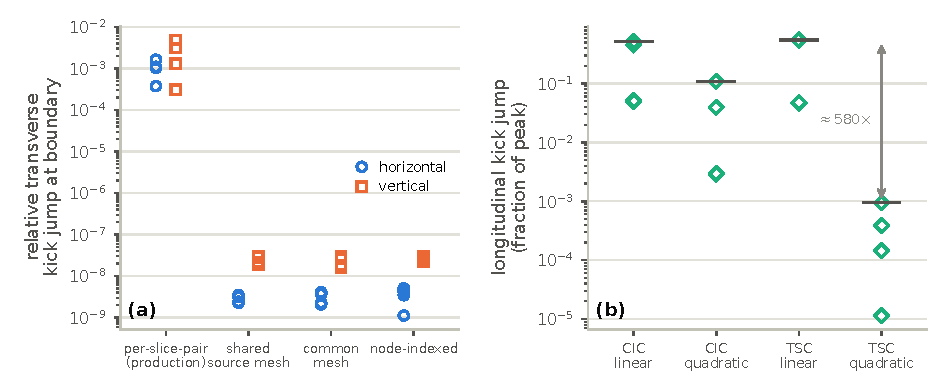
\includegraphics[width=0.95\linewidth]{figs/fig_boundary_jump.pdf}
\caption{Slice-boundary tests for a flat EIC-like source,
seven quantile slices, $64^2$ cells, and $2\times10^5$ macroparticles.
Each jump is divided by the peak magnitude of the corresponding exact kick
over the scan.  (a) Four frozen-source grid constructions and a node-indexed
live-source control; each marker is one of two source slices at one of two
central boundaries.  The ``node production'' values use the full scheduled
node calculation.  (b) Frozen-source longitudinal
jumps for four assignment/interpolation combinations.  Diamonds are the same
four samples and horizontal bars mark their maxima.}
\label{fig:bjump}
\end{figure}
\FloatBarrier

\subsection{Interpretation}
\label{sec:fieldvsdyn}

The decomposition explains why a finer mesh need not produce a quieter
multi-turn calculation: it resolves a more accurate mean field and also more
of the finite-particle structure.  It does \emph{not} by itself predict
emittance growth, diffusion, or a required particle count, which depend on
temporal correlations, resampling, damping, and lattice dynamics.  We
therefore use Eq.~\eqref{eq:error_split} as a solver diagnostic and validate
multi-turn observables independently in Section~\ref{sec:validation}.
\FloatBarrier
\section{Validation of the collective physics}
\label{sec:validation}

No single comparison can establish the correctness of a strong--strong
program, so the validation is deliberately layered.  Structural identities
test map conventions; analytic Gaussian fields and the independent spectral
solver test transverse kicks; ensemble and mesh studies test numerical error;
and CPU/CUDA comparisons test backend consistency.  Vlasov theory and the
unmodified BeamBeam3D code then test collective dynamics.  A historical EIC
case illustrates the complete application chain but is not counted as
source-pinned validation because its full raw provenance was not retained.
AI tools assisted implementation and analysis; their output is not treated as
evidence.  Each scientific claim is instead tied to an
analytic limit, an independent implementation, a convergence or ensemble
test, or recomputation from archived numerical records.

Unless stated otherwise, the Octopus PIC comparisons in this section use
Float64, CIC deposition, the integrated Green function, second-order field
differences, linear longitudinal interpolation, pair-indexed extrema grids,
and centroid-centered normal-quantile slicing.  The luminosity anchor instead
sets $\kbb=0$ and specifies its CIC luminosity grid independently.

Short CPU/CUDA regression tests provide a bounded backend check.  Two-turn
soft-Gaussian and standard-PIC cases with 1024 macroparticles per beam, three
slices, and (for PIC) a $32^2$ mesh passed coordinate and luminosity relative
tolerances of $10^{-10}$.  Eight one-collision Gaussian-subtracted cases with
6000 macroparticles per beam, five slices, and a $64^2$ mesh passed the
coordinate vector-norm and luminosity criteria at relative tolerance
$10^{-9}$ and coordinate absolute tolerance $10^{-18}$; six also passed the
stricter elementwise coordinate bound.  These are short regression tests, not
a claim of bitwise or long-term backend equivalence.

\subsection{Structural checks}
\label{sec:eicdemo}

Structural checks establish the map conventions before collective observables
are compared.  Decreasing the centered-difference step from
$3\times10^{-7}$ to $3\times10^{-8}$ lowers the symplectic defects of the thin
synchro-beam and analytic Gaussian maps from
$7.91\times10^{-8}$/$4.24\times10^{-8}$ to
$7.90\times10^{-10}$/$4.24\times10^{-10}$, consistent with second-order
finite-difference truncation.  The crossing boost and inverse compose to
identity to $8.3\times10^{-19}$, and the strong--strong models approach their
frozen-source limits as source energy increases.

\subsection{Coherent modes and the Yokoya factor}
\label{sec:yokoya}

The coherent $\sigma/\pi$ dipole spectrum is a direct test of
self-consistent distribution dynamics
\citep{MellerSiemann1981,YokoyaKoiso1990,Alexahin2002}.  Two identical round
beams collide at one IP with $\xi=0.005$, tunes $(0.31,0.32)$, one
longitudinal slice, and no crossing angle.  One beam starts at
$0.1\sigma$ offset.  We extract the sum and difference mode tunes from
8192-turn Hann-windowed centroid spectra using parabolic peak interpolation
and form
\begin{equation}
  \Lambda=\frac{Q_\pi-Q_\sigma}{\xi}.
  \label{eq:yokoya}
\end{equation}
A rigid-bunch model gives $\Lambda=1$; the linearized Vlasov result is about
$1.2144$ for round Gaussian beams
\citep{YokoyaKoiso1990,HerrPieloni2014}.

At the stated $128^2$, $0.1\sigma$, 8192-turn setting, three PIC runs give
$\Lambda=(1.1973\pm0.0035,1.2061\pm0.0004)$, where the uncertainties are seed
scatter only.  Figure~\ref{fig:coherent} shows the centroid spectra and the
fitted $Q_\sigma$ and $Q_\pi$ for one representative seed.  One-at-a-time changes, averaged over the same three seeds, quantify the
larger numerical
envelope: $128^2\!\rightarrow256^2$ shifts $(\Lambda_x,\Lambda_y)$ by
$(+0.0045,+0.0030)$, $0.1\sigma\!\rightarrow0.025\sigma$ by
$(+0.0070,+0.0060)$, and 8192 to 16384 turns by
$(-0.0002,-0.0031)$.  A zero-padded diagnostic attributes much of the last
vertical shift to three-bin interpolation and FFT-bin phase.  Thus the robust
claim is a round-beam factor near 1.20--1.21, not a three-decimal continuum
limit.  Gaussian-subtracted PIC gives the value listed in
Table~\ref{tab:yokoya}, while soft-Gaussian gives
$\Lambda=(1.096,1.100)$: evolving moments recover part
of the shift above the rigid value but omit distribution-shape feedback
\citep{Yokoya2000}.

An exploratory flat-beam calculation has fixed $\xi_x=0.005$ and therefore
$\xi_y=0.0556$; it is not used as validation of the linear flat-beam limit.

\subsection{Cross-code comparison with BeamBeam3D}
\label{sec:bb3d}

The same physical configuration --- round beams, one IP, single slice, no
crossing angle, $10^5$ particles, $128\times128$ transverse grid, 8192 turns
--- was run without source modification in BeamBeam3D
\citep{Qiang2004BeamBeam3D} (V1.0, commit \code{50d01d8}), compiled with GNU
Fortran 11.5.0 and OpenMPI 4.1.1.
Independent builds and full reruns reproduced the reported centroid outputs.
The executable
logs a realized single-slice strength of $0.0049932095$.  Table~\ref{tab:yokoya}
uses the predeclared nominal denominator $\xi=0.005$; using the logged value
would give $(\Lambda_x,\Lambda_y)=(1.1991,1.2115)$ instead of
$(1.1974,1.2098)$, a 0.136\% normalization change.  With the nominal convention,
the differences from the three-seed Octopus mean are $0.00016$ in $x$ and
$0.00371$ in $y$, and less than $4\times10^{-6}$ in $Q_\sigma$.  The codes
share no source but implement the same CIC/integrated-Green method.

\begin{table}[pos=h]
\centering
\caption{Fixed-setting round-beam Yokoya factors
$\Lambda=(Q_\pi-Q_\sigma)/\xi$ (8192 turns, $10^5$ macroparticles/beam,
$\xi=0.005$, one slice).  PIC reports mean $\pm$ seed SD for three runs, not
total numerical uncertainty; the soft-Gaussian and Gaussian-subtracted rows
are three-seed means and BeamBeam3D is a single run.  BeamBeam3D uses the
nominal denominator.  The Vlasov reference is 1.2144.}
\label{tab:yokoya}
\begin{tabular}{lccc}
\toprule
solver & $\Lambda_x$ & $\Lambda_y$ & assessment \\
\midrule
soft-Gaussian            & 1.096 & 1.100 & below Vlasov value (closure) \\
PIC $128^2$              & $1.1973\pm0.0035$ & $1.2061\pm0.0004$ & fixed setting \\
Gaussian-subtracted PIC $64^2$ & 1.198 & 1.206 & max.\ distance 1.34\% \\
BeamBeam3D               & 1.1974 & 1.2098 & independent code \\
\bottomrule
\end{tabular}
\end{table}

\begin{figure}[!ht]
\centering

\includegraphics[width=0.84\linewidth]{figs/fig_coherent_fft.pdf}
\caption{Round-beam PIC centroid spectra for one of three seeds
($8192$ turns, $10^5$ macroparticles/beam, $\xi=0.005$, one slice).
Each plane is normalized to its largest sum- or difference-mode amplitude.
Dashed lines mark the fitted $Q_\sigma$ and $Q_\pi$; the other seeds give the
scatter in Table~\ref{tab:yokoya}.}
\label{fig:coherent}
\end{figure}
\FloatBarrier

\subsection{Multi-slice cross-code benchmark}
\label{sec:msbench}

A five-slice benchmark exercises the synchro-beam map and longitudinal
kick.  Both codes use $\sigma_z/\beta^*=0.5$, $|Q_s|=0.01$,
$\xi=0.005$, $5\times10^4$ macroparticles per beam, and 4096 turns.
Synchrotron modulation produces the line structure shown in
Fig.~\ref{fig:msbench}.  With the displayed symmetric Hann window, the
estimator searches $[Q_0-0.004,Q_0+0.010]$ and refines local maxima above
1\% of the in-band maximum by a three-bin parabola.  Under that prescription,
the noise-excited Octopus and coherently kicked BeamBeam3D horizontal traces
each contain six peaks.  Frequency-rank pairing gives median/maximum
$|\Delta Q|=(1.20,3.84)\times10^{-4}$, with the maximum equal to 1.6 raw
FFT bins.  Varying the peak threshold or window changes the accepted peak
count, and the two traces use different excitation protocols.  Figure
\ref{fig:msbench} therefore establishes similar horizontal spectral structure,
not one-to-one mode identity.

\begin{figure}[!ht]
\centering
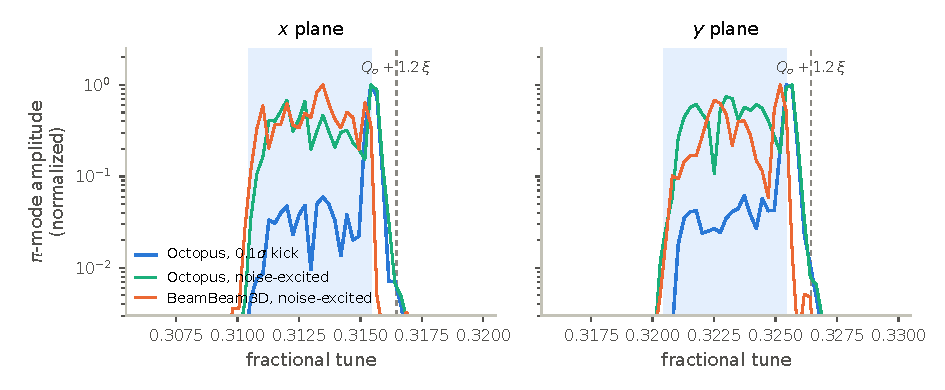
\includegraphics[width=0.78\linewidth]{figs/fig_multislice_spectra.pdf}
\caption{Five-slice normalized difference-mode spectra ($5\times10^4$
macroparticles/beam, $\sigma_z/\beta^{*}=0.5$, $|Q_s|=0.01$, $\xi=0.005$,
4096 turns).  Shading spans $[Q_\sigma,Q_\sigma+\xi]$ and the dashed line marks
$Q_\sigma+1.2\xi$.  The noise-excited Octopus and coherently kicked BeamBeam3D
horizontal traces each contain six peaks under the stated estimator; the
comparison supports similar structure, not common mode identities.}
\label{fig:msbench}
\end{figure}
\FloatBarrier

\subsection{Crossing-angle and crab-cavity luminosity anchor}
\label{sec:lumanchor}

For equal frozen round Gaussians ($\sigma_x=\sigma_y=100\,\mu$m,
$\sigma_z=2$~cm, $\beta^{*}=0.5$~m), 15 normal-quantile slices, and
$2\times10^5$ macroparticles per beam, a half crossing angle of
$\theta_c/2=12.5$~mrad gives Piwinski parameter
$\phi=(\sigma_z/\sigma_x)\tan(\theta_c/2)=2.5$.  The analytic luminosity
factor is $R_\phi=(1+\phi^2)^{-1/2}=0.371391$
\citep{HerrMuratori2006}.  Five paired particle seeds give
$L/L_0=0.371950\pm0.000272$ (sample standard deviation), while ideal crab
cavities restore $L/L_0$ to $1.000000\pm0.000010$.  A one-seed scan over 1, 7,
15, and 31 slices and $128^2$/$256^2$ grids spans 0.37147--0.37195, with no
monotonic slice trend.  The production estimator retains particle midpoint
coordinates; a centroid-only 15-slice quadrature gives 0.369274 and is not its
finite-slice target.  This checks relative boost/crab/luminosity geometry, not
absolute luminosity.

\subsection{Historical EIC emittance application}
\label{sec:emitbench}

The preceding tests isolate field and collective-mode behavior.  To exercise
the complete multi-turn chain, we retain one historical Octopus and one
historical BeamBeam3D run for a head-on, 15-slice collision at parameters
adapted from the EIC design \citep{EICCDR2021}: 10~GeV electrons
($\xi_e=(0.088,0.100)$, $\beta^*=(0.55,0.056)$~m,
$\sigma^*=(106,9.5)\,\mu$m) against 275~GeV protons
($\xi_p=(0.0094,0.0094)$, $\beta^*=(0.80,0.072)$~m,
$\sigma^*=(95,8.5)\,\mu$m), a $128^2$ mesh, $10^5$ macroparticles per beam,
and 8192 turns.  The proton side uses the design optics; the electron side
departs from it ($\beta^*_x=0.55$ versus $0.45$~m, $\epsilon_y=1.61$ versus
$1.3$~nm), so the spot sizes are unequal and $\xi_{e,x}$ and $\xi_p$ differ
from the design values $\xi_e=(0.072,0.10)$, $\xi_p=(0.012,0.012)$.  The electron damping times are shortened from
$(4000,4000,2000)$ to $(400,400,200)$ turns in $(x,y,z)$ so that the run
approaches an equilibrium; the proton remains undamped.  Octopus uses
electron/proton populations $1.7203\times10^{11}$/$0.6881\times10^{11}$,
whereas the archived BeamBeam3D decks use
$1.72\times10^{11}$/$0.69\times10^{11}$.  Octopus also uses Gaussian Philox
excitation while BeamBeam3D uses variance-matched uniform excitation.  The
transverse tunes are $(0.08,0.14)$ for electrons and $(0.228,0.210)$ for
protons in both codes, but Octopus uses synchrotron tunes
$(-0.069,-0.01)$ for the electron/proton beams while BeamBeam3D uses
$(+0.069,+0.01)$ under the same linear-map sign convention.  Initial
macroparticles are generated independently, and each code uses its native
longitudinal slicing and adaptive field domains.  The case therefore tests
how the two program chains behave under related, but not matched, inputs.

These trajectories predate the frozen source-state record used elsewhere in
this article.  The BeamBeam3D decks, log, and raw outputs and the reduced
Octopus emittance series survive, but the original executable-to-trajectory
identity is incomplete; the native Octopus HDF5 file, converter, command, log,
environment, and source identity were not retained.  Table~\ref{tab:emitbench}
and Fig.~\ref{fig:emitbench} are therefore a transparently historical,
qualitative application comparison, not source-pinned validation or an exactly
replayable result.

\begin{table}[H]
\centering
\caption{Historical EIC emittance application (15 slices, 8192 turns,
$10^5$ macroparticles/beam; one run per code under nonidentical inputs).
Values are late-time means over common sampled turns
$6144$--$8176$ (128 records). Electron values are relative to the design
emittance; undamped proton values are relative to each run's first record.}
\label{tab:emitbench}
\begin{tabular}{llccc}
\toprule
beam & plane & Octopus & BeamBeam3D & difference \\
\midrule
\multicolumn{5}{l}{\emph{electron: equilibrium relative to design emittance}}\\
electron & $x$ & $+11.03\%$ & $+10.76\%$ & $+0.27$~pp \\
electron & $y$ & $+4.66\%$  & $+3.56\%$  & $+1.10$~pp \\
\midrule
\multicolumn{5}{l}{\emph{proton: growth relative to each code's initial value}}\\
proton & $x$ & $+0.576\%$ & $+0.643\%$ & $-0.067$~pp \\
proton & $y$ & $+1.092\%$ & $+1.182\%$ & $-0.090$~pp \\
\bottomrule
\end{tabular}
\end{table}

\begin{figure}[!ht]
\centering

\includegraphics[width=0.95\linewidth]{figs/fig_eic_emittance.pdf}
\caption{Emittance evolution in the historical EIC application
($10^5$ macroparticles/beam, 15 slices, $128^2$ mesh). Electron curves are
relative to design emittance and include shortened radiation damping and
excitation; undamped proton curves are relative to each code's initial sample.
Blue and orange denote Octopus and BeamBeam3D; solid and dashed lines denote
the $x$ and $y$ planes.}
\label{fig:emitbench}
\end{figure}
\FloatBarrier

The late-time electron means differ by $0.27$ percentage points (pp) in $x$
and $1.10$~pp in $y$; proton growth differs by $0.067$ and $0.090$~pp.  These
retained curves exhibit the same qualitative evolution and comparable
late-time changes in this demanding case.  Because there is one realization
per code, the stated input differences, and incomplete run provenance, the
comparison is physical application context, not validation of identical
dynamics or a measure of statistical cross-code uncertainty; the
$1.10$~pp electron-$y$ difference is about 31\% of BeamBeam3D's induced
equilibrium excess.

Taken together, the source-pinned tests span map structure, field accuracy,
coherent modes, multi-slice spectra, and crossing geometry; the historical EIC
application adds long-term emittance evolution without extending that
validation claim.
Matched ensemble-level code comparison, the linear wide-plane flat-beam limit,
and the crab-compensated coherent-mode family of \citet{OhmiCrossing2017}
remain outside the present study.

\FloatBarrier
\section{Performance}
\label{sec:cuda}

\subsection{CUDA execution strategy}

Because each encounter modifies its slices, all slice pairs cannot collide
concurrently.  Octopus partitions the collision-time schedule into
wavefronts whose pairs share no slice.  CUDA kernels access particles through
slice index lists, without temporary gather/scatter copies.  Charge and force
planes use batched FFTs; persistent workspaces and aspect-ratio-keyed Green
functions avoid per-pair allocation and kernel construction.

Other high-volume operations follow the wavefront: fused two-level reductions
set source and target bounds, both longitudinal planes are deposited together,
and normalization, spectral multiplication, finite differences, and gathering
remain on the device.  Scheduling and data movement change, but both backends
implement the same ordered collision algorithm.  Floating-point reduction
order is backend-dependent, so agreement is tested with stated tolerances and
is not claimed to be bitwise identity.

\subsection{Benchmark and scaling}

The benchmark uses 2.56 million electron and 1.024 million proton
macroparticles, 15 quantile slices per beam (225 slice pairs and 450
directed field evaluations), a $128^2$ CIC mesh, integrated Green function,
linear longitudinal interpolation, pair-indexed adaptive grids, and the EIC
crab-crossing lattice \citep{EICCDR2021}.  The timed turn includes luminosity
output every turn and two HDF5 moment observers.  FP64 measurements use the
source commit identified below on an
NVIDIA RTX~4500 Ada (24~GB, driver 580.119.02), CUDA.jl 6.2.1, Julia 1.12.4,
and a single host Julia thread on an Intel Xeon Gold 6430.

\begin{table}[pos=h]
\centering
\caption{Measured GPU wall time per turn, including the observers described in
the text.  Entries are means $\pm$ sample SD across independent process
medians after warm-up (five processes for the nominal case and three for the
other cases).  Scaling windows include one HDF5 observer flush.}
\label{tab:performance}
\begin{tabular}{lccc}
\toprule
configuration & total particles & mesh & median s/turn \\
\midrule
half population & $1.79\times10^6$ & $128^2$ &
$0.2048\pm0.0009$ \\
nominal, coarse mesh & $3.58\times10^6$ & $64^2$ &
$0.2612\pm0.0007$ \\
nominal & $3.58\times10^6$ & $128^2$ &
$0.3067\pm0.0070$ \\
nominal, fine mesh & $3.58\times10^6$ & $256^2$ &
$0.5106\pm0.0019$ \\
double population & $7.17\times10^6$ & $128^2$ &
$0.4786\pm0.0093$ \\
\bottomrule
\end{tabular}
\end{table}

At the nominal point, five process means give $0.3129\pm0.0071$~s/turn;
the mean of the corresponding process medians is
$0.3067\pm0.0070$~s/turn.
Multiplying the process-mean $0.3129$~s/turn by $10^5$ gives an arithmetic
extrapolation of 8.69 GPU-hours.  The robust process-median scaling values are 0.2048 and
0.4786~s/turn when both particle populations are halved or doubled, and
0.2612 and 0.5106~s/turn for nominal $64^2$ and $256^2$ meshes
(Table~\ref{tab:performance}).
A separate idle Julia CUDA context occupied about 3.2~GiB during the
measurements but showed zero GPU utilization.  The results are elapsed times
on one shared-host device, not a multi-architecture performance model.
They are also conservative with respect to data-center hardware: the
weak--strong companion case at $1.02\times10^6$ macroparticles, with the
same every-turn luminosity and moment output, measured 3.9~ms/turn on an
NVIDIA A100 against about 105~ms/turn on this device (the timing record is
archived in \code{docs/history/weak\_strong\_cuda\_luminosity\_2026\_08\_11.md}
at the cited source commit), a gap that largely reflects the A100's FP64
pipeline running at 1:2 of its FP32 rate, versus 1:64 on this
workstation-class GPU, with the A100's higher memory bandwidth also
contributing.  If the same FP64-throughput advantage carries over to the
kernel-dominated strong--strong phases, the nominal case projects to well
below 0.2~s/turn on an A100-class GPU; this is a projection from the
measured weak--strong pair, not a measurement.

\section{Summary}
\label{sec:summary}

Octopus combines four complementary transverse field models,
six-dimensional multi-slice collision physics, and GPU execution in one
strong--strong framework.  The error analysis shows why accuracy cannot be
described by mesh size alone: refinement reduces mean-field bias but can expose
more finite-particle fluctuation.  Assignment-consistent Gaussian subtraction
lowers the near-Gaussian discretization error, while node-indexed meshes remove
the boundary mismatch introduced by independently adapted slice-pair domains.

The validation connects these numerical results to collective observables.
PIC-family and BeamBeam3D round-beam coherent factors lie within 1.42\% of the
Vlasov reference, the largest same-setting Octopus--BeamBeam3D difference is
0.31\%, and the
five-slice spectra show similar horizontal structure.  The historical
15-slice EIC comparison adds a demanding example of complete multi-turn
emittance evolution in both programs.  Its nonidentical inputs and incomplete
raw provenance make it qualitative application context, not source-pinned
validation or a statistical-equivalence study.  At EIC production scale, 3.58 million
macroparticles and 15 slices advance in about 0.31~s/turn on one workstation
GPU, and well below 0.2~s/turn projected on data-center FP64 hardware.  Together, the solver-specific error budget, layered validation, and
measured throughput support practical strong--strong studies in the tested
domain.

\section*{Code and data availability}

Octopus is released under the MIT license at
\url{https://github.com/xud929/Octopus.jl}~\citep{OctopusSoftware2026}.  The
source state evaluated for this manuscript is commit
\href{https://github.com/xud929/Octopus.jl/commit/01e97c58afcacec46a337284c2799a1571dccb23}
{\code{01e97c58afca}}
(\code{v0.1.11-423-g01e97c5}, branch \code{paper-cpc}).
Octopus requires Julia 1.12; the CUDA backend uses CUDA.jl 6.2, with FFTW,
HDF5/JLD2, and SpecialFunctions as the remaining core dependencies, resolved
by the committed project environment (\code{julia --project=.}).  A
simulation constructs the two beams and lattice maps and selects the field
model by passing one of the four solver objects
(\code{PICPoissonSolver}, \code{GaussianPoissonSolver},
\code{SpectralPoissonSolver}, \code{GaussianPICPoissonSolver}) to the
collision element; all four implement the shared \code{collide!} interface,
and \code{test/examples/strong\_strong\_tracking.jl} is the worked
strong--strong example.  The unit and regression test suite runs with
\code{julia --project=. -e 'using Pkg; Pkg.test()'}.  BeamBeam3D is cited at the unmodified independent
source commit used for the source-pinned comparisons
\citep{BeamBeam3DSoftware2024}.  The
Gaussian-subtracted configuration evaluated here is specified in
Table~\ref{tab:solver_capabilities} and remains experimental.  Input decks and
selected raw and reduced numerical records, and the reduction and plotting
programs underlying the reported figures and numerical tables are provided in
the public reproducibility repository
\url{https://github.com/xud929/2026_octopus_cpc}, which also records the
per-dataset regeneration standing against the cited source state.  For the historical EIC comparison,
the archive contains BeamBeam3D decks, log, and raw outputs and the reduced
Octopus series, but not the native Octopus HDF5 output or the complete original
run identities.  The supplied Octopus runner at the cited source state enables
a new calculation; it does not retrospectively source-identify the plotted
historical curves.

\section*{Declaration of generative AI and AI-assisted technologies in the manuscript preparation process}

Claude (Anthropic) and Codex (OpenAI) assisted with derivations,
implementation, tests, numerical analysis, and editing.  The authors checked
derivations against limiting cases and source conventions, required executable
tests for code changes, recomputed reported values from archived data, and made
all scientific decisions.  The authors take full responsibility for the
software, analysis, and manuscript.

\section*{Declaration of competing interest}

The authors declare no competing financial interests or personal
relationships that could have appeared to influence the work reported in
this paper.

\printcredits

\section*{Acknowledgments}

The authors thank the BeamBeam3D authors for making their code publicly
available, which enabled the cross-code comparison of
Section~\ref{sec:bb3d}.  Work supported by Brookhaven Science Associates,
LLC under Contract No.\ DE-SC0012704 with the U.S. Department of Energy.
The sponsor's role was limited to financial and institutional support; the
authors retained responsibility for study design, data collection, analysis
and interpretation, manuscript preparation, and the decision to submit.

\bibliographystyle{model1-num-names}
\bibliography{ref}

\end{document}
